\newcommand{\TRESicmin}{1.85\xspace}
\newcommand{\TRESicmax}{3.10\xspace}
\newcommand{\TRESicNoveNoveMin}{1.62\xspace}
\newcommand{\TRESicNoveNoveMax}{3.33\xspace}
\newcommand{\TRESnZero}{26\xspace}


Foram retiradas 200 amostras, sem reposição, com tamanhos 4, 8, 16, 30 e 100, 
dentre os 4986 alunos que possuíam um valor definido para a variável Renda.
A população possuí média de ${\UMx}$ para a variável Renda, com desvio padrão de
${\UMsd}$. A \autoref{tab:q1} apresentam os valores esperados da média amostral
e seu respectivos desvios padrões.

\begin{table}[h]
\centering
\caption{Valores das médias amostrais para a variável \textit{Renda}}
\label{tab:q1}
\vspace{0.5em}
\begin{tabular}{l r r r}
	\toprule
	\textbf{\specialcell{c}{Tamanho da\\Amostra}} & \textbf{Média} & \textbf{\specialcell{c}{Desvio\\Padrão}} & \textbf{$\frac{\sigma}{\sqrt{n}}$}\\
	\midrule
	$4$       & ${\UMxQuatro}$   & ${\UMsdQuatro}$   & ${\UMsdeQuatro}$   \\
	$8$       & ${\UMxOito}$   & ${\UMsdOito}$   & ${\UMsdeOito}$   \\
	$16$      & ${\UMxDezesseis}$  & ${\UMsdDezesseis}$  & ${\UMsdeDezesseis}$  \\
	$30$      & ${\UMxTrinta}$  & ${\UMsdTrinta}$  & ${\UMsdeTrinta}$  \\
	$100$     & ${\UMxCem}$ & ${\UMsdCem}$ & ${\UMsdeCem}$ \\
	\bottomrule
\end{tabular}
\end{table}

\subsection{(item a)}
A medida que se aumentou o tamanho da amostra, de 4 para 16, o resultado se aproximou à media populacional.
Porém para amostra de tamanho 30 e 100, a média amostral se distanciou da média populacional.


\subsection{(item b)}
Sim, as amostras retiradas confirmam a afirmação. Conforme indicado na \autoref{tab:q1}, os valores 
de desvio padrão das amostras são próximos aos valores de $\frac{\sigma}{\sqrt{n}}$ e para a amostra de tamanho 100, 
são exatamente iguais.

\subsection{(item c)}

\begin{figure}[h]
\begin{minipage}{0.49\textwidth}
	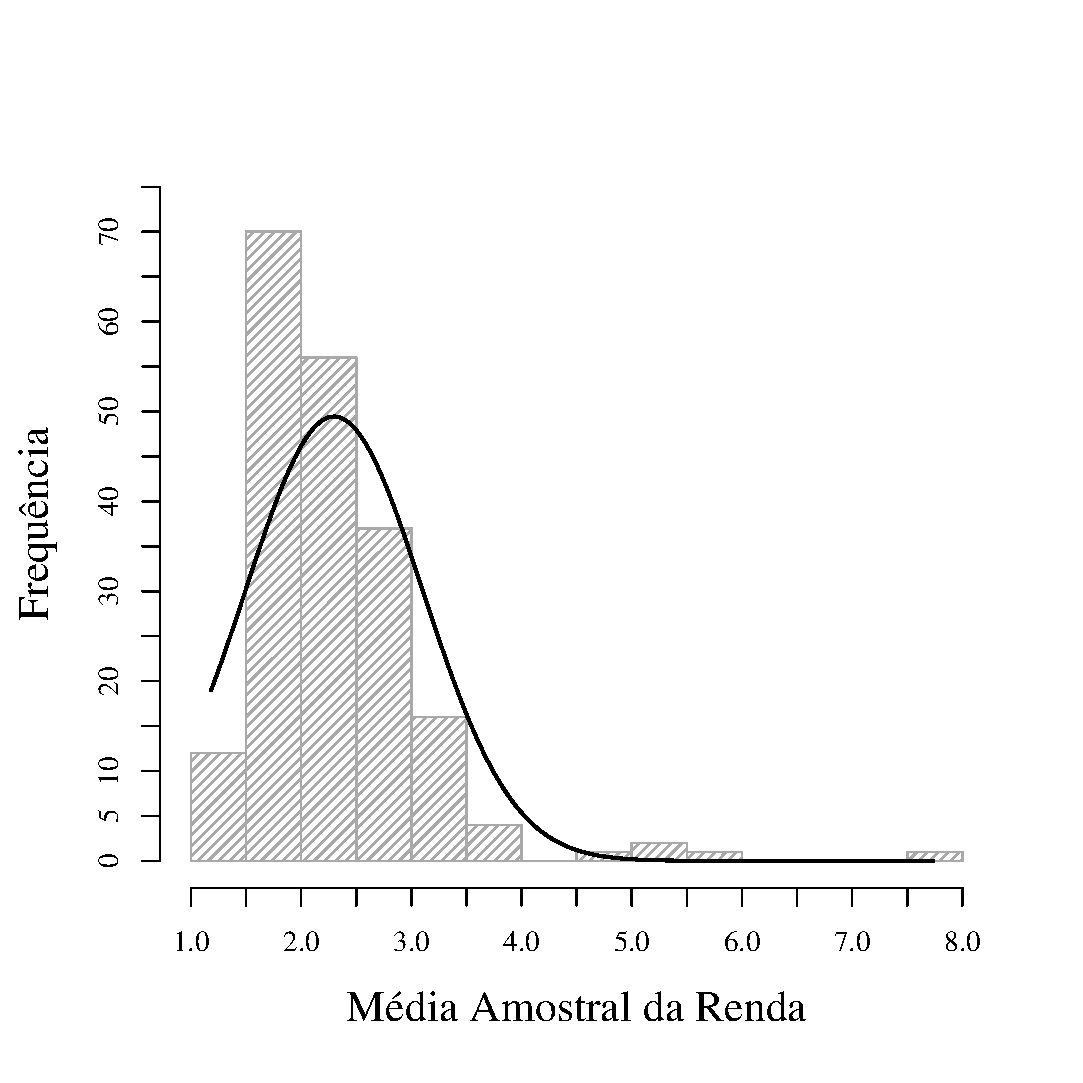
\includegraphics[width=\linewidth]{questao1/histogram_renda_m4.eps}
	\caption{Amostra de tamanho 4}
	\label{fig:m8}
\end{minipage}
\begin{minipage}{0.49\textwidth}
	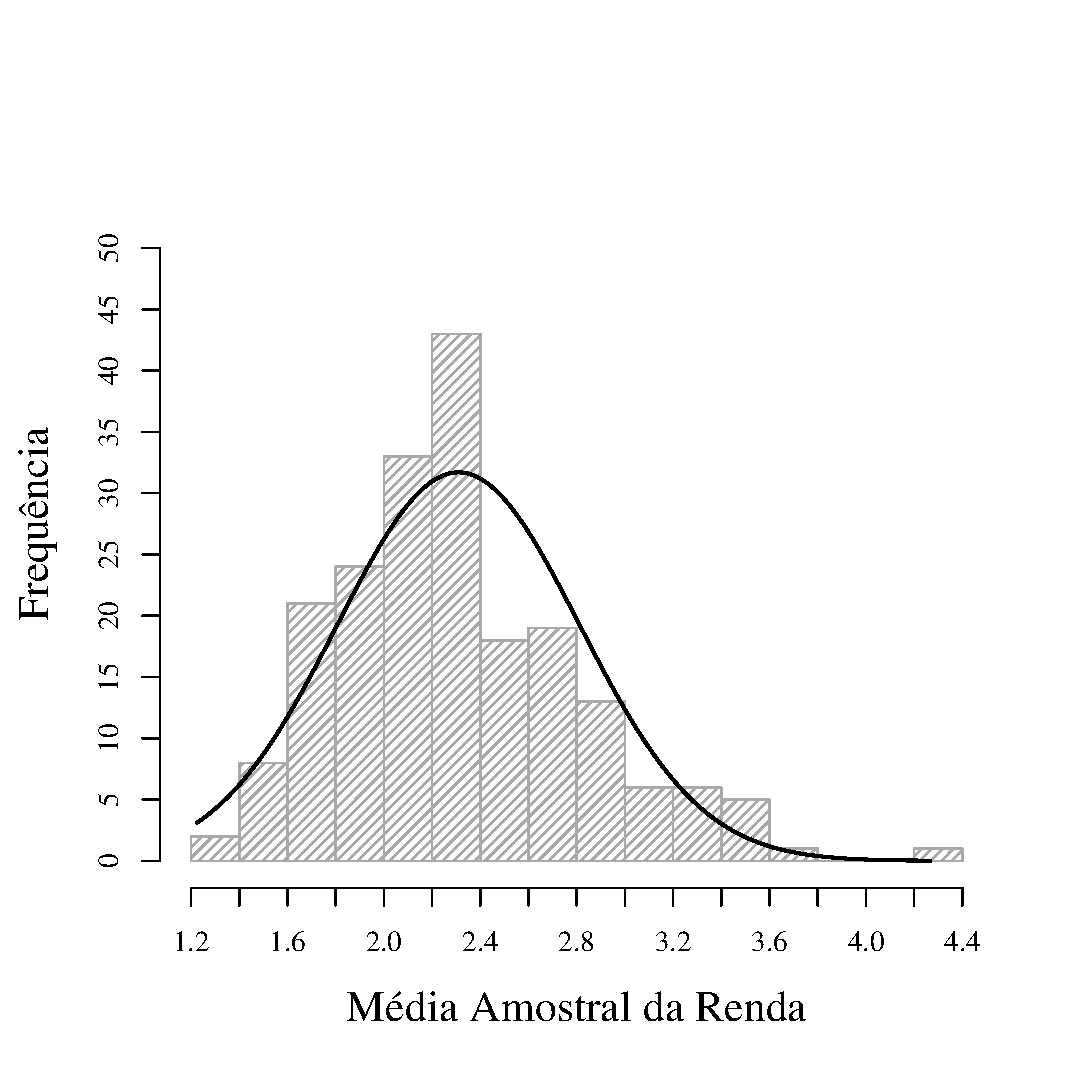
\includegraphics[width=\linewidth]{questao1/histogram_renda_m8.eps}
	\caption{Amostra de tamanho 8}
	\label{fig:m8}
\end{minipage}
\end{figure}

\begin{figure}[h]
\begin{minipage}{0.49\textwidth}
	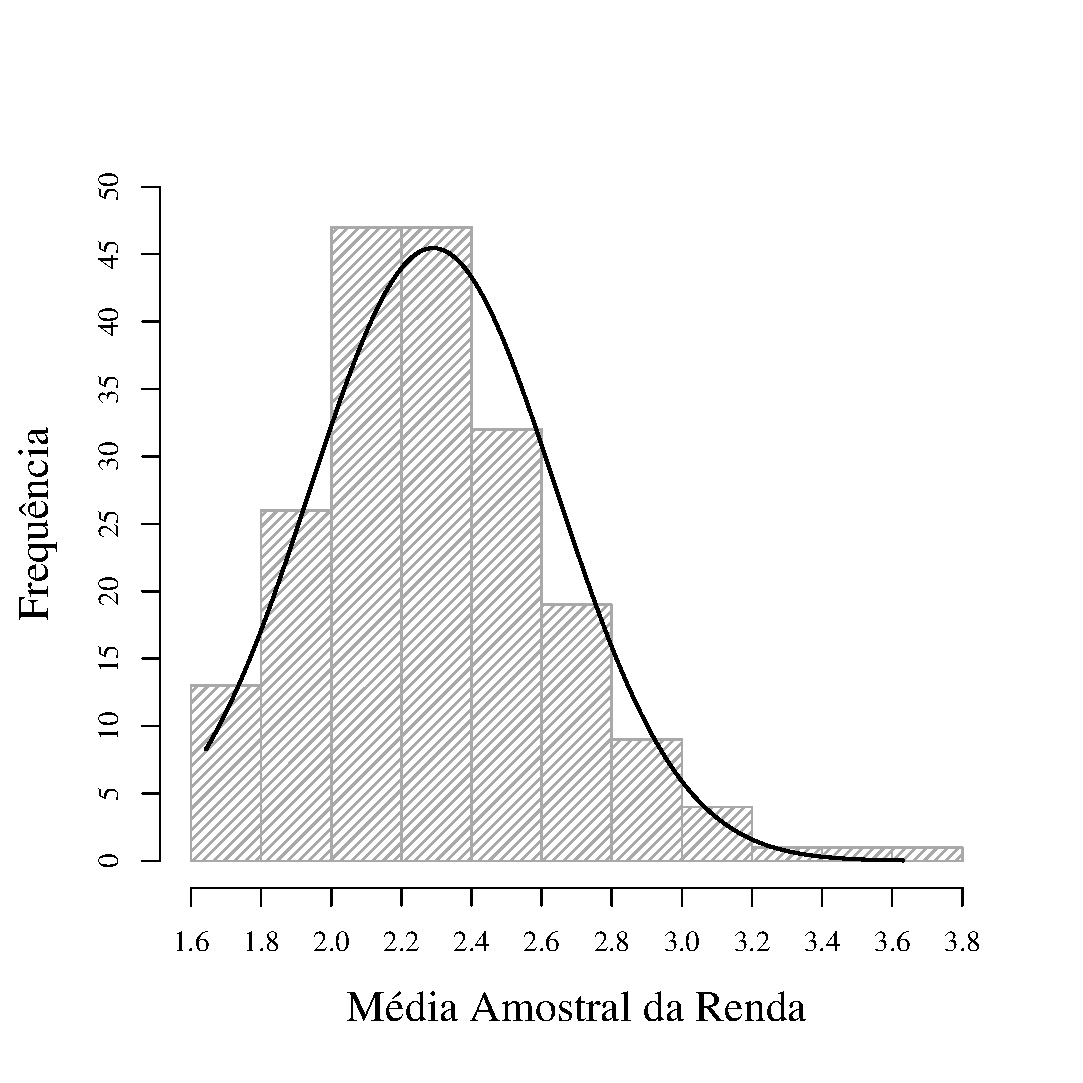
\includegraphics[width=\linewidth]{questao1/histogram_renda_m16.eps}
	\caption{Amostra de tamanho 16}
	\label{fig:m16}
\end{minipage}
\begin{minipage}{0.49\textwidth}
	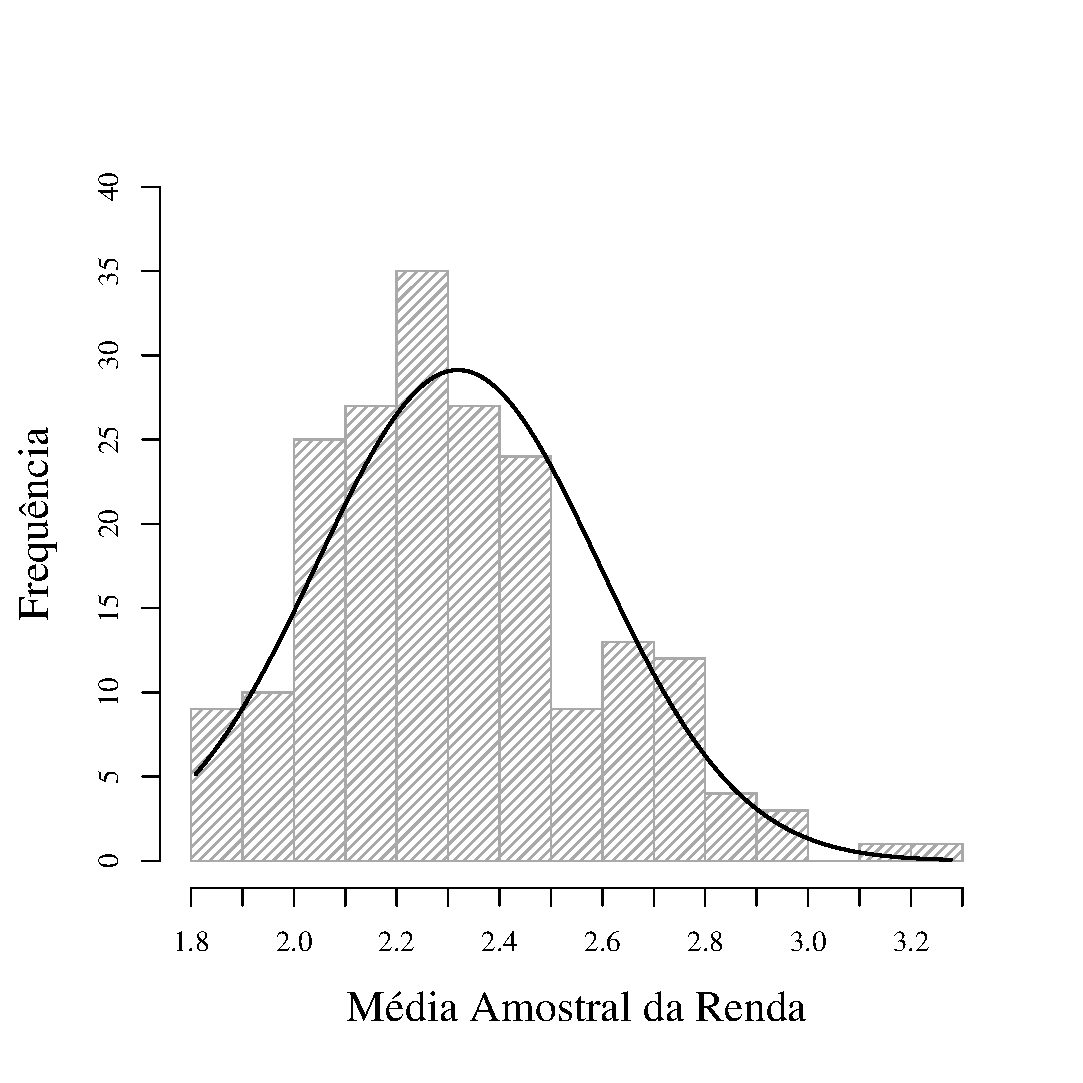
\includegraphics[width=\linewidth]{questao1/histogram_renda_m30.eps}
	\caption{Amostra de tamanho 30}
	\label{fig:m30}
\end{minipage}
\end{figure}

\begin{figure}[h]
\centering
	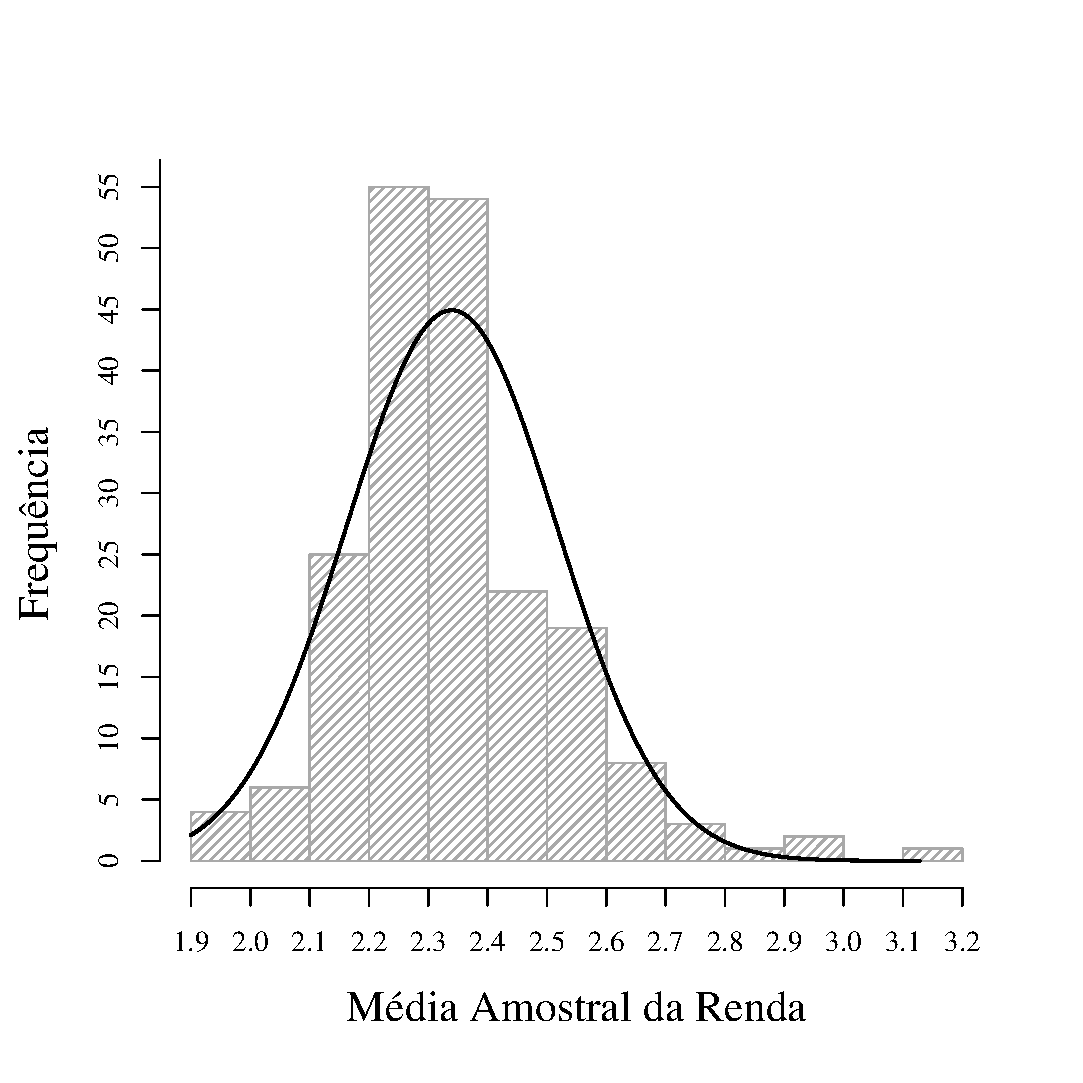
\includegraphics[width=0.49\textwidth]{questao1/histogram_renda_m100.eps}
	\caption{Amostra de tamanho 100}
	\label{fig:m100}
\end{figure}

\FloatBarrier
